\documentclass{beamer}
\usetheme{madrid}

\setbeamercolor{postit}{fg=black, bg=yellow!30}


\usepackage{amssymb}
\usepackage{amsmath}
\usepackage{amsthm}
\usepackage{stmaryrd}
\usepackage{wasysym}
\usepackage{tabularx}
\usepackage{graphicx}
%\usepackage{tikz}
\usepackage{listings}  % Formatiert Code
\usepackage{xcolor}
\usepackage{listings}

\lstset{escapeinside={<@}{@>}}

%\usetikzlibrary{arrows,automata}

\newcommand{\bla}{\bigwedge\limits}
\newcommand{\blo}{\bigvee\limits}

\newcommand{\la}{\land}
\newcommand{\lo}{\lor}
\newcommand{\lr}{\rightarrow}
\newcommand{\llr}{\leftrightarrow}
\newcommand{\lp}{\oplus}
\newcommand{\p}{\text{potenz}}
\newcommand{\R}{\Rightarrow}
\newcommand{\n}[1]{\overline{{#1}}}
\newcommand{\bb}[1]{\mathbb{{#1}}}

\newcommand{\step}[1]{&& \left|\ {#1} \right.}
\newcommand{\e}[2]{{#1}\cdot 10^{{#2}}}
\newcommand{\blue}{\textcolor{blue}}
\newcommand{\red}{\textcolor{red}}
\newcommand{\green}{\textcolor{magenta}}

\setbeamertemplate{enumerate item}{(\alph{enumi})}
\setbeamertemplate{enumerate subitem}{(\roman{enumii})}

%	\newcounter{enumtemp}
%	\setcounter{enumtemp}{\theenumi}
%	-
%	\setcounter{enumi}{\theenumtemp}

\title{TikTok and News Sites Extraction}
\subtitle{Mastodon}
\author{Gruppe 1}
\institute{}
\date{\today}

\begin{document}
\begin{frame}
    \titlepage
\end{frame}
\begin{frame}
    \frametitle{Mastodon}
    Was ist Mastodon?
    \begin{itemize}
        \item free and open-source social network
        \item sehr ähnlich zu Twitter
        \begin{itemize}
            \item Man kann 'Toots' posten
            \item Es gibt Hashtags, die trenden
            \item Man kann anderen Nutzern folgen
        \end{itemize}
    \end{itemize}
    ~\\
    Wichtiger Unterschied zu Twitter: Mastodon ist \blue{dezentral}.
    \begin{itemize}
        \item Es gibt keinen Hauptserver, den alle User nutzen.
        \item Stattdessen gibt es Instanzen, auf denen User Accounts anlegen und posten können.
        \item Instanzen sind isoliert funktionsfähig.
        \item Können aber auch mit anderen Instanzen interagieren.
    \end{itemize}
\end{frame}
\begin{frame}
    \frametitle{Funktionen}
    Das Programm hat folgende Funktionen:
    \begin{itemize}
        \item Eine Liste von Instanz-Domains in einer Datenbank speichern.
        \item Für jede der Instanzen Toots fetchen und speichern.
        \begin{itemize}
            \item Welche Attribute der Toots gespeichert werden, ist auszuwählen.
            \item Toots sollen nach verschiedenen Eigenschaften filterbar sein.
        \end{itemize}
        \item Für jede Instanz Statistiken zur Antwortzeit angeben.
    \end{itemize}
\end{frame}
\begin{frame}
    \frametitle{IDs in Mastodon}
    Für das Fetchen der Toots, muss man die IDs von Mastodon verstehen.
    \begin{center}
        bis zu \blue{6 bytes millisecond timestamp} + 2 bytes unique sequence data
    \end{center}
    Entsprechend können Toots wie folgt chronologisch sortiert werden.
    \begin{itemize}
        \item Sortiere nach Größe: Neuere Toots haben längere IDs.
        \item Sortiere Lexikographisch.
    \end{itemize}
    Aus der Toot-ID ist also auch der Postzeitpunkt berechenbar.
\end{frame}
\begin{frame}
    \frametitle{IDs in Mastodon}
    \begin{center}
        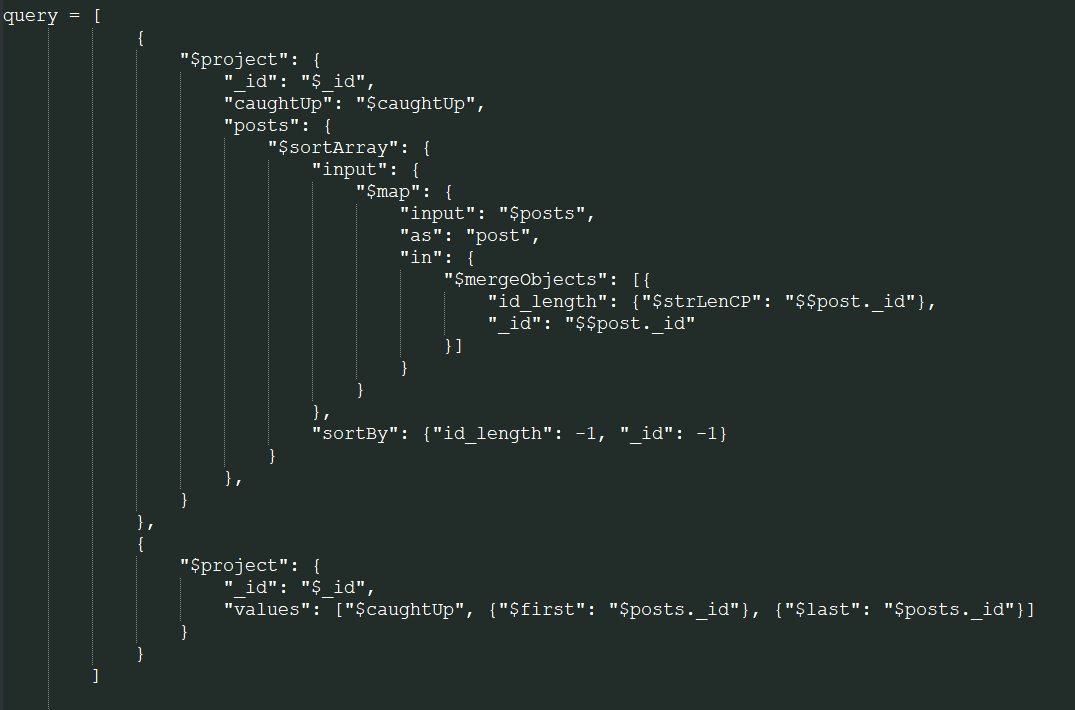
\includegraphics[width=\textwidth]{w.png}
    \end{center}
\end{frame}
\begin{frame}
    \frametitle{Fetchen von Toots}
    Der folgende Link gibt 40 Toots aus der Instanz 'mastodon.social'.
    \begin{center}
        \blue{
            \href{https://mastodon.social/api/v1/timelines/public?limit=40}
            {https://mastodon.social/api/v1/timelines/public?limit=40}
        }
    \end{center}  
    Dazu kann man eine \red{ID} als Parameter geben.
    \begin{center}
        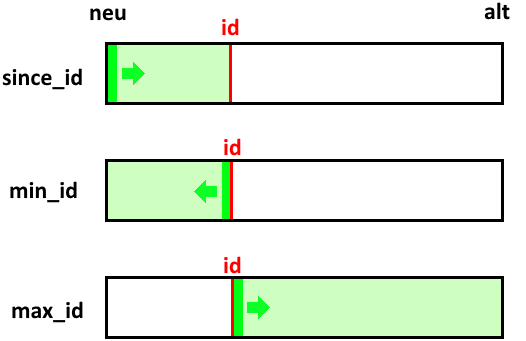
\includegraphics[width=0.6\textwidth]{b.png}
    \end{center}    
\end{frame}
\begin{frame}
    \frametitle{Fetchen von Toots}
    Dazu kann man eine \red{ID} als Parameter geben.
    \begin{center}
        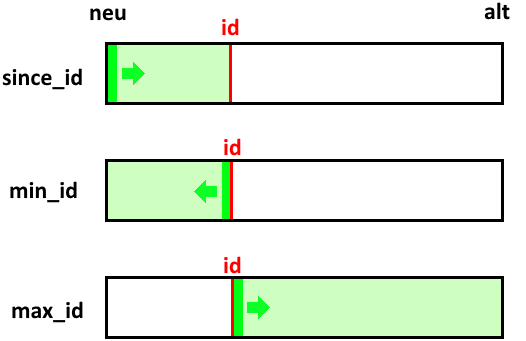
\includegraphics[width=0.6\textwidth]{b.png}
    \end{center}   
    \begin{center}
        \blue{https://mastodon.social/api/v1/timelines/public?limit=40\&max\_id=1111}
    \end{center}  
    Gibt die neusten Toots, die eine \red{ID} $>$ 1111 haben, also \blue{älter} sind.
\end{frame}
\begin{frame}
    \frametitle{Probleme}
    Da Mastodon dezentral ist, hängt das Fetchen von einzelnen Instanzen ab.
    \begin{itemize}
        \item Manche Instanzen brauchen Bewerbungen für die Registrierung.
        \item Einzelne Attribute der Toots können fehlen.
        \item 5xx Fehler und unterschiedliche Antwortzeiten. 
    \end{itemize}
\end{frame}

\end{document}